\documentclass[assignment01_Solutions]{subfiles}

\IfSubStr{\jobname}{\detokenize{Solutions}}{\toggletrue{solutions}}{\toggletrue{solutions}}

\fancypagestyle{firstpage}

{\rhead{Assignment 1 \linebreak \textit{Version: \today}}}

\title{Assignment 1: Bayes' Rule}
\author{Machine Learning}
\date{Fall 2019}

\begin{document}

\maketitle
\thispagestyle{firstpage}


TODO: make these more concrete based on Connor's comment in the course feedback survey. (note: Perhaps breaking these down in more detail when we get to a particular problem / reading is better).

\begin{learningobjectives}
\bi
\item Gain familiarity with key ideas in ML (with a focus on probabilistic methods).
\item Formal definition of a probability.
\item Bayes' Rule
\item Applications of Bayesian Inference
\ei
\end{learningobjectives}

\section{Motivation}
We’ve talked about the idea of uncertainty a lot in this class.  For instance, we learned about the logistic regression model, which when given an input, computes the probability that the output is 1.  This model embraces the idea that it is uncertain in its predictions and uses the concept of a probability to express those uncertainties.  We’ve also seen examples of models that don’t fit the data perfectly.  For example, the plot in Figure~\ref{fig:lineofbestfit} shows a line of best fit that doesn't go through all of the data.  The fit might be imperfect because we don't have the right model (a form of uncertainty) or because the thing we are trying to predict is inherently random in some way (another form of uncertainty).
\begin{marginfigure}
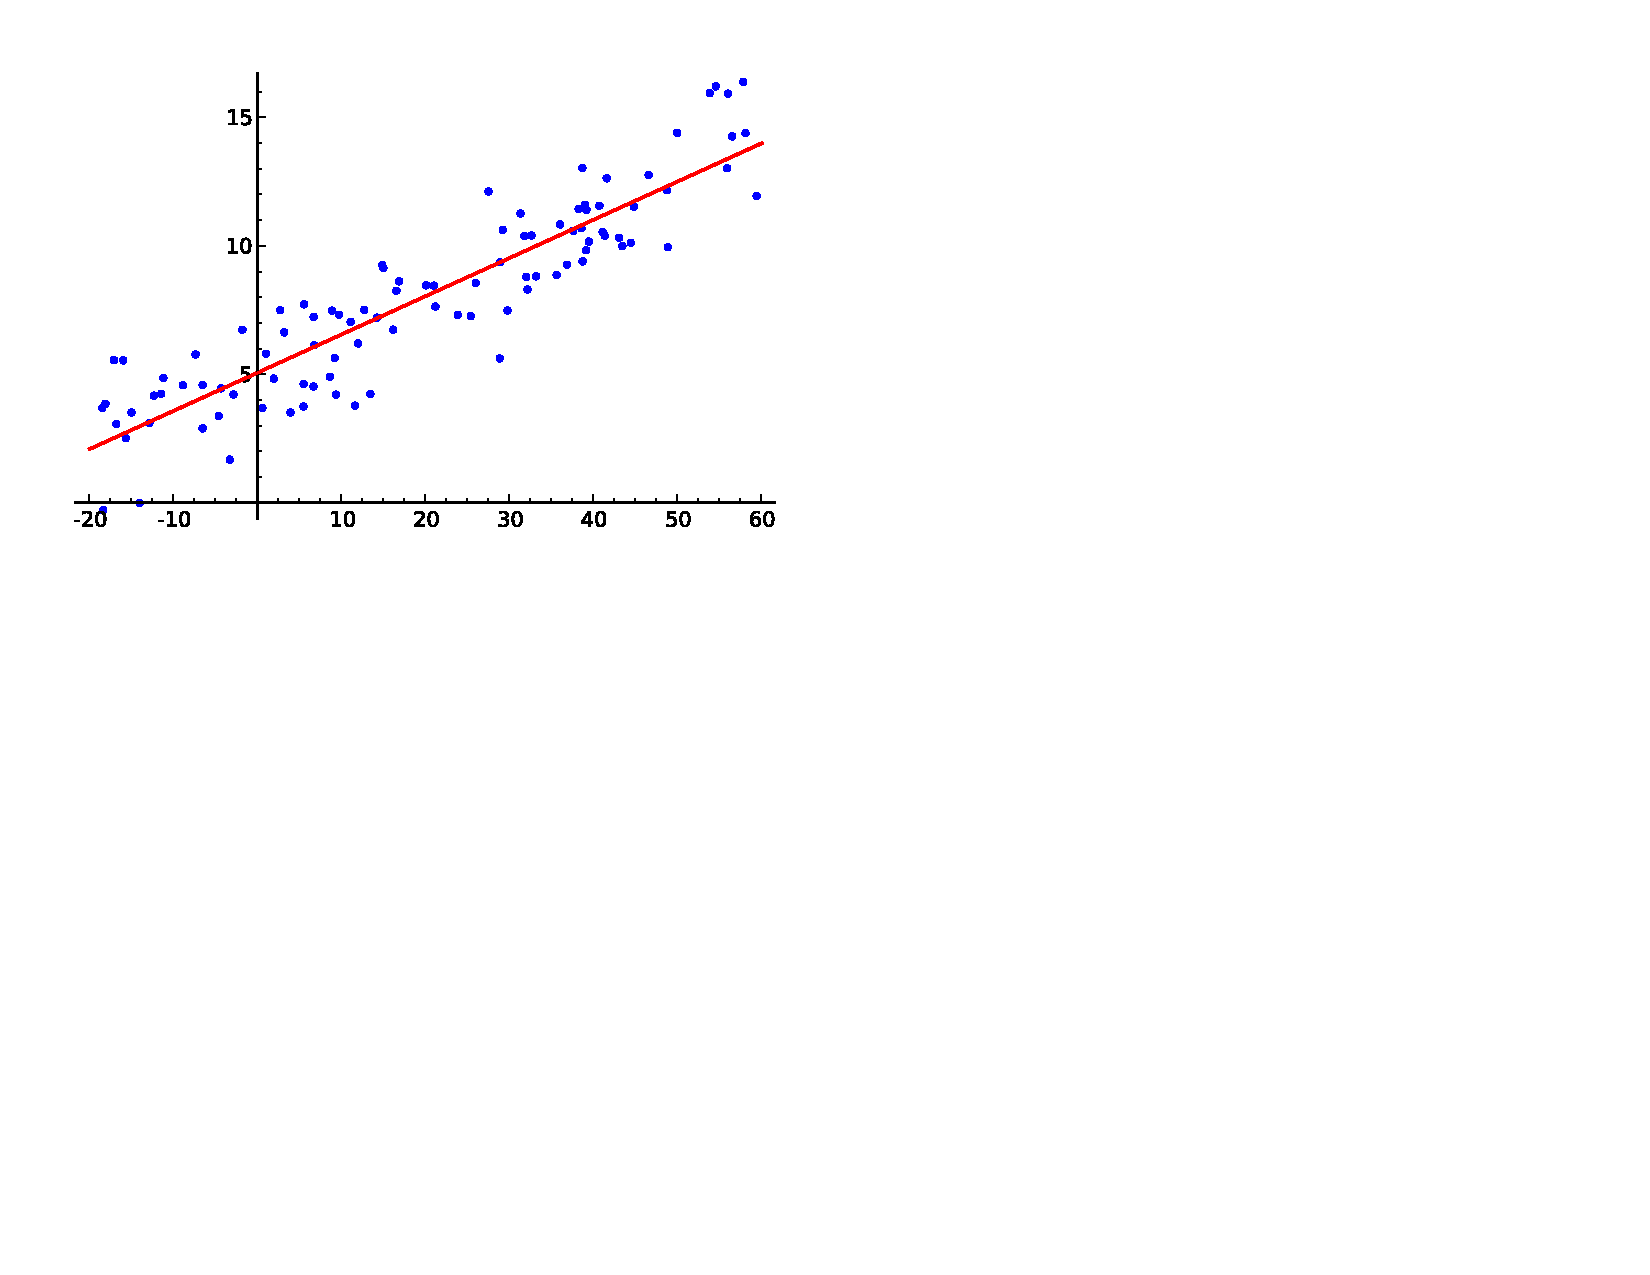
\includegraphics[width=\linewidth]{figures/line_of_best_fit.pdf}
\caption{A dataset with one independent variable (x-axis) and one dependent variable.  Also shown is the line of best fit.\label{fig:lineofbestfit}}
\end{marginfigure}


It turns out the probability theory will give us a precise way to define the concept of uncertainty and reason about all the various forms of uncertainty in a unified way.  Formalizing uncertainty in this way will enable us to do a bunch of really cool things with respect to machine learning, including

\bi
\item make more explicit our assumptions about where data comes, the uncertainties present in it, and how uncertainty impacts predictions we might create based on that data.
\item allow us to quantify our confidence in our model.  For example, instead of returning the one best fitting model, we will be able to assign a confidence (a probability) to each possible model being the right model model.
\item give us a way to incorporate prior knowledge into our machine learning models.  This prior knowledge will allow for us to more easily interpret machine learning models.
\item give us powerful tools to reason about fairness and bias in machine learning models.
\ei

\section{Six Big Ideas in (Probabilistic) Machine Learning}
We're going to reprise the Six Big ideas in ML from our very first assignment with a focus on connections to probabilistic machine learning.  Our intent is to provide a larger framework for you to interpret the content you are learning.  Could potentially point to \href{https://www.nature.com/articles/nature14541.pdf}{this article in Nature Reviews}.


The \href{https://docs.pymc.io/nb_examples/index.html}{pymc examples} are also super cool (e.g., \href{https://docs.pymc.io/notebooks/GP-MaunaLoa.html}{GP Mauna Loa})

\subsection*{Idea 1: Probabilistic Methods Help Us Understand Learning in Artificial Systems and Biological Systems}

\subsection*{Idea 2: Probabilistic Methods Can Illuminate Hidden Structures}

\bi
\item Phylogenetic trees
\item \href{https://homes.cs.washington.edu/~rao/indus.html}{Indus Script}
\ei


\subsection*{Idea 3: Probabilistic Methods Give Us a Language for Reasoning about Algorithmic Fairness}

\subsection*{Idea 4: Probabilistic Methods Allow Us to Attach Confidences to Our Predictions}

\href{https://docs.pymc.io/notebooks/GP-MaunaLoa.html}{Mauna Loa CO2 example}

\subsection*{Idea 5: Probabilistic Methods Allow for Learning More Interpretable Models}

https://towardsdatascience.com/what-is-bayesian-statistics-used-for-37b91c2c257c

\subsection*{Idea 6: Probabilistic Methods Let you Learn Hierarchies of Models}
TODO (clustering or topic modeling?)


\subsection*{notes: other ideas}
\bi
\item Decision-making under uncertainty
\item \href{https://arxiv.org/pdf/1809.10756.pdf}{Probabilistic Programming?} (Note: there is an example of inverse computer graphics that is cool).  Here is \href{https://www.youtube.com/watch?v=DImI6l_0yiM}{one that references 3D computer vision}.  Here is probably the \href{http://mrkulk.github.io/www_cvpr15/}{clearest version}.  Another \href{cool example}{https://arxiv.org/pdf/1607.08128.pdf}.  This one is \href{https://science.sciencemag.org/content/sci/360/6394/1204.full.pdf}{really insane (from Science)}.   It uses a few images to predict what the scene would look like from another viewpoint.
\item Compression?
\ei

\begin{exercise}[\faShareAlt~(60 minutes)]
Now, we want to hear from you!  
Choose one of the big ideas above and write a short response to it.  Your response could incorporate something surprising you read, a thought-provoking question, your personal experience, an additional resource that builds upon or shifts the discussion.  We hope that this reflection will help scaffold class discussions and get you thinking about your interests in the big space that is ML.  Also, you have license from us to customize the structure of your response as you see fit.  As a rough guide, you should aim for a response of a 1-2 paragraphs.

\begin{boxedsolution}
There's no one right answer here!
\end{boxedsolution}
\end{exercise}

\section{Probability}

Hopefully the previous section left you feeling excited to learn more about the theory that might underlie these sorts of models and applications.  Next, we'll be taking our first steps towards learning this theory.

\subsection{Intuition}
Most of us are used to thinking that events can be probabilistic, that is we can attach some probability to whether or not they occur.  Take for example flipping a coin.  We could think of the event that the coin comes up heads as having probability 0.5.  That is, there is an even chance that it happens versus doesn’t happen.  Further, we can talk about events as being observable if we are able to ultimately know whether or not they occurred.  For instance, whether a coin comes up heads is an observable event since you can ultimately observe the outcome of the flip.  In contrast, some events would be considered unobservable if they are unable to be directly ascertained by human senses.  A classic example of this would be whether a scientific theory is true or not.  It is impossible to directly observe whether the theory is true, but you might be able to observe events that are consistent or inconsistent with the theory.

\vspace{1em}
\begin{exercise}[(10 minutes)]
Come up with some examples of observable events that are probabilistic in nature.  For each event, either provide the probability or explain what factors would determine the probability.  Some potential ideas to get you going: sporting events, elections, weather, etc.

\begin{boxedsolution}
TODO
\end{boxedsolution}

\end{exercise}

\subsection{Formal Definition}

Next, we'll define more formally\sidenote{this is not the full definition of a \href{https://en.wikipedia.org/wiki/Probability_space}{probability space} used in modern mathematics.  For the purposes of most people that \emph{use} probability theory on actual problems, this definition is needlessly complex.  Use the following link if you want a more \href{https://m.tau.ac.il/~tsirel/dump/Static/knowino.org/wiki/Probability_space.html}{in-depth discussion of the parts of the formal definition that are tricky} (our expectation is that you won't want this discussion!).} what we mean by a probability.  Having this formal definition will give us the ability to useful rules for manipulating and reasoning about probabilities.  To define the concept of a probability, we'll need to specify two ingredients.
\subsection{Events}

The first is the notion we need to fine is an \textbf{event}.  Think of an event as something that may or may not occur in response to some random process.  For instance, we could define the event that a coin comes up heads when it is flipped.  We often use capital letters to indicate events.  Since we've been using capital letters to also represent matrices, in our materials we'll use a cool mathy-looking calligraphic font to represent events.  For instance, we might use the symbol $\mathcal{H}$ to refer to the event that a coinflip comes up heads. It's important to emphasize that a single random process can have many associated events.   For instance, for the coin flip example we might also define $\mathcal{T}$ to be the event that the coin comes up tails.

Further, events don't necessarily have to be mutually exclusive.  For instance, we might define the $\mathcal{R}_h$ to indicate the event that the Republican party controls the majority in the house of representatives following the 2020 election and $\mathcal{D}_s$ to indicate the event that the Democratic party controls the majority in the senate following the 2020 election.  Both (or none) of these events could occur.

\subsection{Probability Measure Function}
The probability measure function assigns a probability to the occurrence of any particular event.  We can think of this probability measure as a function that takes as input an event and outputs a probability.  For instance, $p(\mathcal{E})$ provides the probability that event $\mathcal{E}$ occurs according to probability measure $p$.  All probability measure functions must satisfy the following properties.

\bi
\item $0 \leq p(\mathcal{E}) \leq 1$ (the probability of an event ranges from 0 (for an impossible event) to 1 (an event that will always occur).
\item Given a set of $n$ events $\mathcal{E}_1, \mathcal{E}_2, \ldots, \mathcal{E}_n$ that are disjoint (i.e., no two can occur simultaneously)
\begin{align}
p(\mathcal{E}_1~\mbox{or}~\mathcal{E}_2~\mbox{or}~\ldots~\mbox{or}~\mathcal{E}_n) = \sum_{i=1}^n p(\mathcal{E}_i) \label{eq:probunion} \enspace .
\end{align}


The equation above specifies what's sometimes called the union rule of probability.  It states that the probability of 1 of these disjoint events occurring must be equal to the sum of the probability of each of the events occurring.  You will also sometimes see Equation~\ref{eq:probunion} written as

\begin{align}
p(\mathcal{E}_1 \cup \mathcal{E}_2 \cup \ldots \cup \mathcal{E}_n) = \sum_{i=1}^n p(\mathcal{E}_i) \enspace .
\end{align}

If you're not familiar with the symbol $\cup$ it is the symbol for a union of two sets.  The reason you'll sometimes see this is that in the most rigorous definition of a probability space, an event is defined formally as a set (as stated in the margin note earlier in this section, you need not worry about the most rigorous definition in this course).

\item Given a set of (not necessarily disjoint) events $\mathcal{E}_1, \mathcal{E}_2, \ldots, \mathcal{E}_n$ where at least one of these $n$ events must occur
\begin{align}
p(\mathcal{E}_1~\mbox{or}~\mathcal{E}_2~\mbox{or}~\ldots~\mbox{or}~\mathcal{E}_n) = 1 \enspace .
\end{align}
\ei
\subsection{Complement Rule for Probability}

Given the definition of probability detailed above, it follows that if the probability of an event happening is $p(\mathcal{E})$ then the probability of the event \emph{NOT} happening is $1-p(\mathcal{E})$.   The following are common ways of expression this relationship (we'll use Equation~\ref{eq:complement} in this class).  These all say the same thing (the only difference is notation).

\begin{align}
p(\neg \mathcal{E}) &= 1 - p(\mathcal{E}) \label{eq:complement} \\
p(\mbox{not}~\mathcal{E}) &= 1 - p(\mathcal{E}) \nonumber \\
p(\overline{\mathcal{E}}) &= 1 - p(\mathcal{E}) \nonumber \\
p(\mathcal{E}') &= 1 - p(\mathcal{E}) \nonumber
\end{align}

We point out these alternate notations not to confuse you (we'd never do that!) but to help you interpret various external resources you might find on these topics.

\vspace{1em}
\begin{exercise}[(10 minutes)]
Here are some diagnostic questions to make sure that you go the basic ideas. 
\bes
\item Suppose $\mathcal{E}_1, \mathcal{E}_2, \mathcal{E}_3$ are disjoint events.  Further, suppose that one of these events must occur.  Which of the following functions are valid probability measure functions?

\begin{align}
p_1(\mathcal{E}_1)=\frac{1}{10} , p_1(\mathcal{E}_2)=\frac{1}{5}, p_1(\mathcal{E}_3)=\frac{7}{10} \nonumber
\end{align}


\begin{align}
p_2(\mathcal{E}_1)=\frac{11}{10} , p_2(\mathcal{E}_2)=\frac{-1}{10}, p_2(\mathcal{E}_3)= 0 \nonumber
\end{align}



\begin{align}
p_3(\mathcal{E}_1)=\frac{1}{10} , p_3(\mathcal{E}_2)=\frac{1}{5}, p_3(\mathcal{E}_3)=\frac{1}{2} \nonumber
\end{align}



\begin{align}
p_4(\mathcal{E}_1)=1 , p_4(\mathcal{E}_2)=0, p_4(\mathcal{E}_3)=0 \nonumber
\end{align}

\begin{boxedsolution}
$p_1$ is a valid probability measure function since the probabilities add up to 1 and all are non-negative.  $p_2$ is not a valid probability measure function since two of the probabilities are outside of the appropriate range $[0,1]$.  $p_3$ is not a valid probability measure function since the probabilities of the three events add up to less than 1. $p_4$ is a valid probability measure function since the probabilities add to 1 and are in the appropriate range.
\end{boxedsolution}

\item The \href{https://en.wikipedia.org/wiki/Birthday_problem}{Birthday Problem} is a well-known probability problem often used in discrete math courses.  According to the Wikipedia article, the probability that at least two students among the 70 students in machine learning this semester share the same birthday is $0.999$.  What is the probability that no two students share the same birthday?

\begin{boxedsolution}
Notice that the event \emph{no two students share a birthday} only happens when the event \emph{at least two students share a birthday} does not happen.  Therefore, these events are complements.

\begin{align}
p(\mbox{no two students share a birthday}) &= 1 - p( \neg \mbox{no two students share a birthday})  \nonumber\\
&= 1 - p(\mbox{at least two students share a birthday}) \nonumber \\
&= 1 - 0.999  \nonumber\\
&= 0.001  \nonumber
\end{align}
\end{boxedsolution}

\ees
\end{exercise}

\section{Bayes' Rule}

\begin{externalresources}[(60 minutes)]
\begin{learningobjectives}
Note that these learning objectives have been written to be very specific (based on feedback from the course survey).  When you first read them, you probably won't know what they mean in detail.  As you return to them hopefully the more precise statement of these learning objectives will be useful for assessing your understanding of the provided resources.

\bi
\item When Bayes' rule is useful (i.e., when $p(A|B)$ is easier to work with than $p(B|A)$).
\item The idea of a conjoint probability $p(\mathcal{A}, \mathcal{B})$ (note: alternate notations include $p(\mathcal{A}~\mbox{and}~\mathcal{B})$ and $p(\mathcal{A} \cap \mathcal{B})$).
\item The definition of a conditional probability $p(\mathcal{A} | \mathcal{B}) = \frac{p(\mathcal{A}~\mbox{and}~\mathcal{B})}{p(\mathcal{B})}$.
\item The equation for Bayes' rule $p(\mathcal{A} | \mathcal{B}) = \frac{p(\mathcal{B} | \mathcal{A}) p(\mathcal{A})}{p(\mathcal{B})}$.
\item The equation for the product rule $p(\mathcal{A}~\mbox{and}~\mathcal{B}) = p(\mathcal{B}) p(\mathcal{A} | \mathcal{B})$.
\ei
\end{learningobjectives}

Allen Downey (ever heard of him?) wrote an excellent book called Think Bayes that introduces Bayesian analysis.  The \href{http://www.greenteapress.com/thinkbayes/html/thinkbayes002.html}{first chapter} starts with a less formal definition of probability than we gave earlier.  The chapter then gives intuitions around conjoint probability (the probability that multiple events occur simultaneously), conditional probability (the probability that some event occurs conditioned on another event having occurred), and finally to Bayes' rule (a surprisingly easy theorem to derive that allows you to write one conditional probability distribution in terms of another).  The Monty Hall problem in section 1.7 is probably okay to gloss over (see Allen's note at the end of that section for why this is the case).

Allen's treatment of the material is, of course, not the only one out there (we like it for its focus on building intuition and focusing on the key ideas).  Here are some other resources you might consider checking out (they are optional).
\bi
\item \href{https://www.khanacademy.org/partner-content/wi-phi/wiphi-critical-thinking/wiphi-fundamentals/v/bayes-theorem}{Khan Academy Video on Bayes' Theorem} shows some simple applications of Bayes' rule and explains why it is a convenient way to reason about the probability of hypothesis given data).
\item \href{https://www.youtube.com/watch?v=R13BD8qKeTg}{Veritasium Episode on Bayes' Theorem} has a bit more history and philosophy of Bayes' Theorem along with some nice visualizations.  It also includes the presenter walking on a very scenic mountain (for some reason), so there's that if nothing else.
\item I (Paul) ran across \href{https://youtube.com/watch?v=nvqXXlz-rx0}{this example of applying Bayes' rule to a real world problem}.  It was created by a grad school friend of mine and is hilarious (lots of Cat Memes).  I did notice that there is a mistake in the math at the 8:12 mark in the video (he states that $p(\mbox{alarm} | \mbox{no theft}) = 1 - p(\mbox{alarm} | \mbox{theft})$, which is not necessarily the case).  It's still a good video though.
\ei

\end{externalresources}

\begin{exercise}
It would be great to have something.
\end{exercise}

\section{Marginalization Rule for Probabilities}
The application of Bayes' rule often proceeded something like this.  Let's define the event $\mathcal{D}$ as whether or not a person has a disease and $\mathcal{S}$ as the event that a particular symptom is observed.  If we want to know $p(\mathcal{D} | \mathcal{S})$ we can apply Bayes' rule.

\begin{align}
p(\mathcal{D} | \mathcal{S}) &= \frac{p(\mathcal{S} | \mathcal{D}) p(\mathcal{D})}{p(\mathcal{S})} \label{eq:bayesdenominator}
\end{align}

In order to calculate $p(\mathcal{S})$, some of the resources simply gave a number (e.g., in the Khan Academy video you Googled and got this value), used a convenient trick to get it (as in Allen's M\&M example), or used the following calculation (as in the Veritasium and Car Alarm videos).

\begin{align}
p(\mathcal{S}) &= p(\mathcal{D}) p(\mathcal{S}|\mathcal{D}) + p(\neg \mathcal{D}) p(\mathcal{S} | \neg \mathcal{D})
\end{align}

We wanted to revisit this calculation as it is hiding away some pretty powerful and interesting stuff.  This calculation can be derived using the technique of marginalizing a probability measure function.  The basic idea is that you want to compute the probability of some event, $\mathcal{A}$.  However, it may be difficult to directly calculate $p(\mathcal{A})$ instead you can introduce another event, $\mathcal{B}$, and write $p(\mathcal{A})$ as:
\begin{align}
p(\mathcal{A}) &= p(\mathcal{A}, \mathcal{B}) + p(\mathcal{A}, \neg \mathcal{B}) \label{eq:marginal}
\end{align}
In the equation above we sometimes say that we are \emph{marginalizing out} $\mathcal{B}$ (by summing over the two possibilities: that $\mathcal{B}$ occurred and that $\mathcal{B}$ did not occur).

\begin{exercise}[(15 minutes)]
Using Equation~\ref{eq:marginal} and other rules of probability you've learned thus far, show that Equation~\ref{eq:bayesdenominator} is true.

\begin{boxedsolution}
\begin{align}
p(\mathcal{S}) &= p(\mathcal{S}, \mathcal{D}) + p(\mathcal{S}, \neg \mathcal{D}) & \mbox{marginalization property, Eq~\ref{eq:marginal}} \nonumber \\
&= p(\mathcal{D})p(\mathcal{S}|\mathcal{D}) + p(\neg \mathcal{D}) p(\mathcal{S} | \neg \mathcal{D})& \mbox{product rule} \nonumber
\end{align}
Note that it was up to us what order we applied the product rule.  If we had first split out $\mathcal{S}$ when going from line 1 to line 2 of our solution, we would have been left with $p(\mathcal{S})p(\mathcal{D}|\mathcal{S}) + p(\mathcal{S}) p(\neg \mathcal{D} | \mathcal{S})$.  This move wouldn't really make any progress towards a solution (since we still don't know $p(\mathcal{S})$.

\end{boxedsolution}
\end{exercise}

\begin{marginfigure}
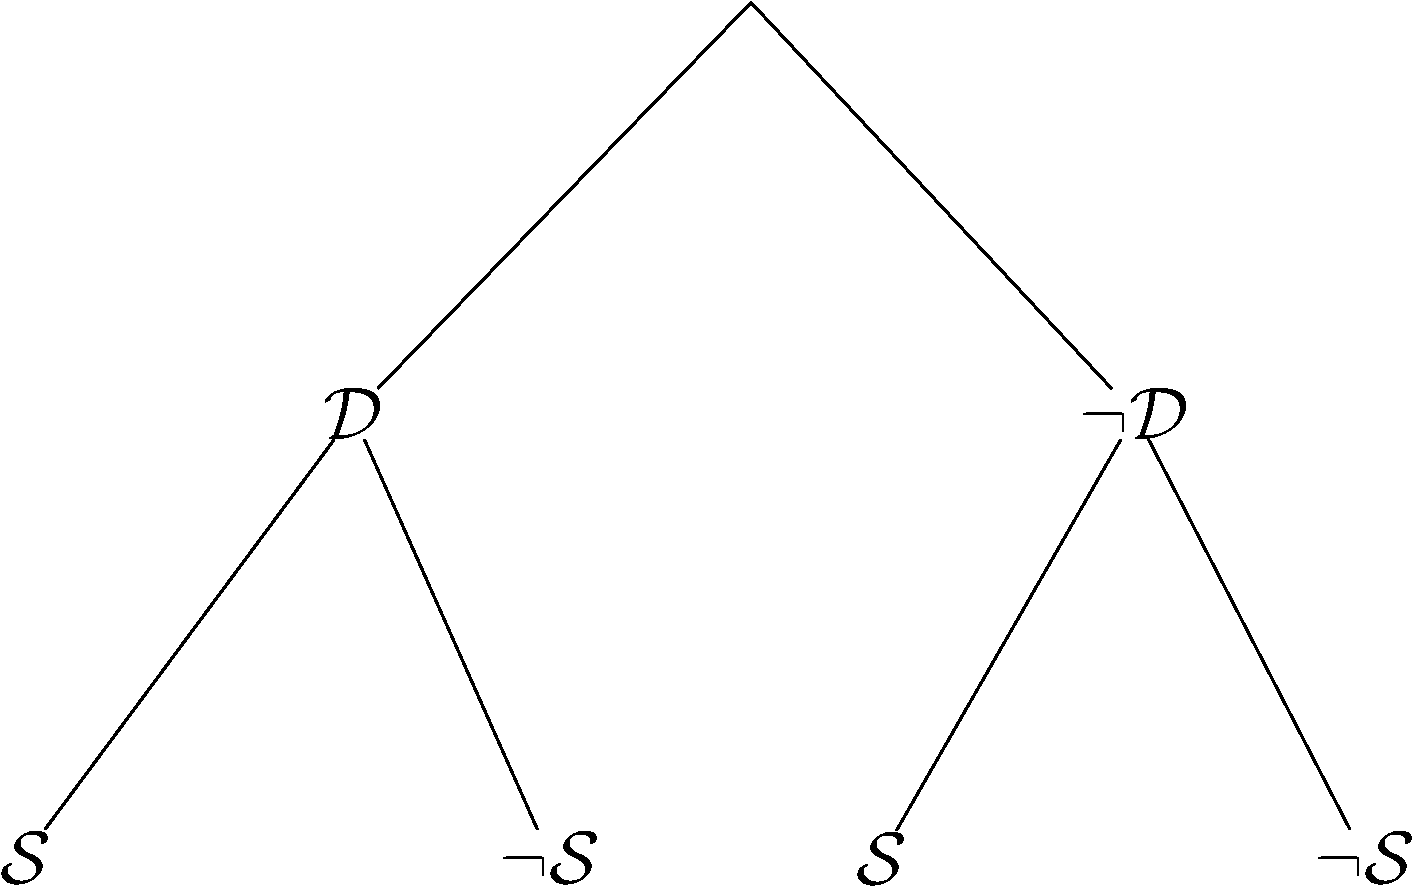
\includegraphics[width=\linewidth]{figures/treenoprobs}
\caption{A tree diagram of the events $\mathcal{D}$ (has a disease) and $\mathcal{S}$ (has a symptom).\label{fig:treenoprobs}}
\end{marginfigure}
Another way to think about marginalization is to draw a tree where you have the event, which you'd like to know the probability of ($\mathcal{S}$ in the previous exercise) and the variable you are marginalizing out ($\mathcal{D}$ in the previous exercise) at the next junction in the tree (see Figure~\ref{fig:treenoprobs}).



Further, we can annotate the arrows with the conditional probability of the event conditioned on the things further up in the tree.

\begin{center}
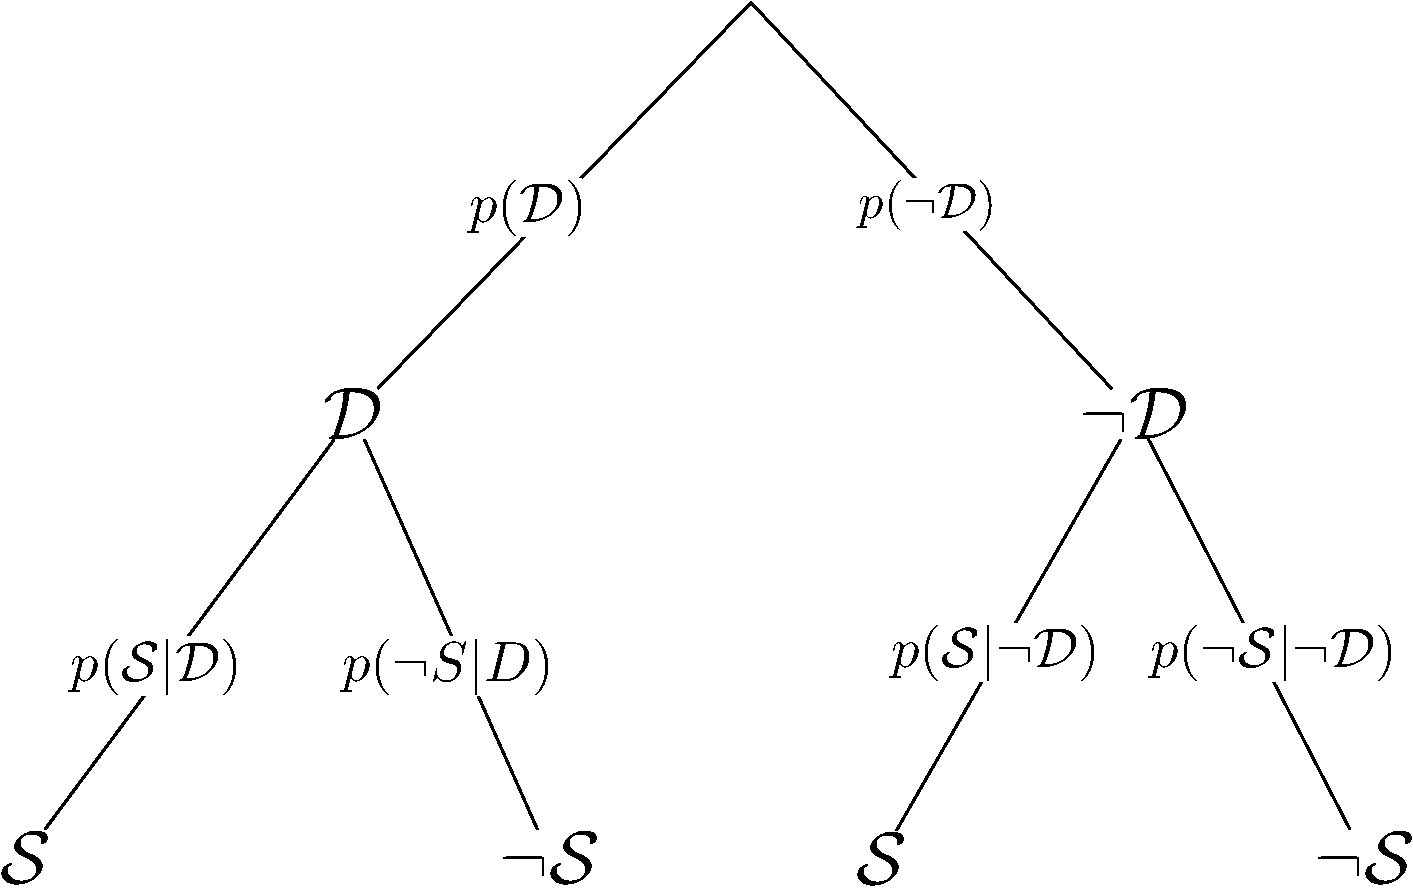
\includegraphics[width=0.6\linewidth]{figures/treeprobs}
\end{center}

If you want to find the probability of anyone joint probability (e.g., $p(\mathcal{D}, \neg \mathcal{S})$), you can follow corresponding path, multiplying probabilities as you go.  For example, from examining the graph above we get
\begin{align}
p(\mathcal{D}, \neg \mathcal{S}) &= p(\mathcal{D}) p(\neg \mathcal{S}|\mathcal{D}) \enspace .
\end{align}

A marginal probability for an event (e.g., $p(\mathcal{S})$) can be found by summing over all paths that arrive at the event.  For example, from examining the graph above we get
\begin{align}
p(\mathcal{S}) &= p(\mathcal{D}) p(\mathcal{S}|\mathcal{D}) + p(\neg \mathcal{D}) p(\mathcal{S}|\neg \mathcal{D})  \enspace .
\end{align}


\begin{exercise}[(20 minutes)]
Do problem 2 from \href{http://wwwf.imperial.ac.uk/~atw/Bayes.pdf}{this assignment}.  They use $\mathcal{E}'$ to refer to the event $\neg \mathcal{E}$.
\begin{boxedsolution}
Solution is embedded in the link.
\end{boxedsolution}
\end{exercise}

\begin{exercise}[(30 minutes)]
Applying Bayes' Rule.  Have a few options for where Bayes could be applied.  Have them pick one of them and figure out an estimate.
\end{exercise}


\section{Random Variables}

We've talked about the concept of an event that captures whether something happens as a result of some random process.  It turns out that it is very useful in machine learning and probabilistic modeling to talk about a variable that captures some quantity that is a result of some random process.  We call this entity a \emph{random variable}.

\begin{externalresources}[(20 minutes)]
Watch the following two videos from Khan Academy on Random Variables.
\bi
\item \href{https://www.khanacademy.org/math/statistics-probability/random-variables-stats-library/random-variables-discrete/v/random-variables}{Khan Academy Video on Random Variables}.
\item \href{https://www.khanacademy.org/math/statistics-probability/random-variables-stats-library/random-variables-discrete/v/discrete-and-continuous-random-variables}{Discrete and Continuous Random Variables} (note: for now we are interested in discrete random variables).
\ei
\end{externalresources}

Now that you have a sense of what a random variable is, we'll introduce the notion of probability mass function (or PMF).  A PMF is a function that assigns a probability to a discrete random variable taking on a particular value as a result of a random process.  We'll use capital, unbolded letters to refer to random variables (e.g., the random variable $X$) and $p(X = k)$ to refer to the probability that $X$ takes on value $k$).

For example, if we were flipping a fair coin 3 times, we might define a random variable $X$ as follows.

\begin{align}
X&= \mbox{the number of coins that come up heads in 3 flips}
\end{align}

The probability mass function is then defined over all possible values that $X$ could possibly take on.  If don't know how we arrived at these values, that is fine.  These are results that can be derived using basic \href{https://en.wikipedia.org/wiki/Combinatorics}{combinatorics} (go take Sarah Spence Adams' class and learn about how to do this).

\begin{align}
p(X=0) &= p(\mbox{0 heads come up} = \frac{1}{8} \nonumber \\
p(X=0) &= p(\mbox{1 heads come up} = \frac{3}{8} \nonumber \\
p(X=0) &= p(\mbox{2 heads come up} = \frac{3}{8} \nonumber \\
p(X=3) &= p(\mbox{3 heads come up} = \frac{1}{8} \nonumber 
\end{align}


\section{Basic Bayes in Python}
\begin{externalresources}[(30 minutes)]
Go through the \href{https://colab.research.google.com/github/mlfa19/assignments/blob/master/Module\%202/01/Assignment_1_Companion_Notebook.ipynb}{assignment 1 companion notebook}.
\end{externalresources}


\end{document}
